\section{Experimental work/analytical investigation/ design}

\subsection{采集数据}
要进行深度学习,所需要的第一步就是采集数据。在本实验中,我们使用了预先从生物实验室制备好的石蜡包埋好的组织切片(鱼的卵巢组织),将其放在HM355s自动切片机上依据切片机的使用手册,以不同的切削角度执行切片操作。记录切削数据。

%在这不要提三个点的鱼的肺泡组织,在后面作为模型二次验证和增强使用。

其中切片机(\autoref{fig:machine})的切片示意图(以牙齿为例) 如\autoref{fig:cutting_machine}所示

\begin{figure}[htbp]
    \centering
    \begin{minipage}{0.48\textwidth}
        \centering
        \includegraphics[width=\textwidth]{./fig/machine.jpg}
        \caption{切片机}
        \label{fig:machine}
    \end{minipage}
    \begin{minipage}{0.48\textwidth}
        \centering
        \includegraphics[width=\textwidth]{./fig/10266_2018_353_Fig1_HTML.jpg}
        \caption{切片机示意图}
        \label{fig:cutting_machine}
    \end{minipage}
\end{figure}
% https://link.springer.com/article/10.1007/s10266-018-0353-6


用于切片的生物组织(示例)如\autoref{label:sample}所示

在切削过程中,从切角为8度开始(如\autoref{fig:machine}中的angle of inclination),每次增加0.5度,直到切角为12度。切片机在切片过程中保持给进速度为25,厚度为1。

在切片完成之后,将切好的不同类型的组织切片放在载玻片上(如\autoref{fig:采集样本})所示,待其晾干后转移至VHX7000显微镜下,通过显微镜对每份样品进行拍照,获取到每份样品的电子图像数据(如\autoref{fig:显微镜})。

\begin{figure}[htbp]
    \centering
    \begin{minipage}{0.3\textwidth}
        \centering
        \includegraphics[width=\textwidth]{./fig/sample.jpg}
        \caption{生物组织切片}
        \label{label:sample}
    \end{minipage}
    \begin{minipage}{0.3\textwidth}
        \centering
        \includegraphics[width=\textwidth]{./fig/采集样本.jpg}
        \caption{采集样本}
        \label{fig:采集样本}
    \end{minipage}
    \begin{minipage}{0.35\textwidth}
        \centering
        \includegraphics[width=\textwidth]{./fig/显微镜.jpg}
        \caption{显微镜}
        \label{fig:显微镜}
    \end{minipage}
\end{figure}

%图片需要后续更改为卵巢的

据此,一共得到9组数据,代表了从8到12每0.5度切角的数据。一共得到约为200张图片,每张图片的分辨率为2880*2160。其中一张(切角9.5度)如\autoref{fig:sample9.5}所示。

\begin{figure}
    \centering
    \includegraphics[width=0.8\textwidth]{./fig/sample9.5.jpg}
    \caption{切角9.5度的样本}
    \label{fig:sample9.5}
\end{figure}

对于这9组数据,需要找到的是在何种切角下,生物组织的完整度最高(质量最好)。因此现在需要将这9组数据根据生物组织的完整度进行重新标注。

根据刀片切割对生物组织的影响,我们将生物组织的完整度分为五个类别,分别为:horizental line, vertical line, slope, other, normal。其中horizental line代表显著的以水平白线为瑕疵的样本,vertical line代表显著的以竖直白线为瑕疵的样本,slope代表图像采集中存在明显的角度(不利于观察),other代表其他瑕疵(如采集中存在明暗显著差别的色块),normal代表正常的生物组织样本。这五类标签的示例图片如下所示。

\begin{figure}
    \centering
    \begin{minipage}{0.45\textwidth}
        \centering
        \includegraphics[width=\textwidth]{./fig/sample_1/horizental_line.jpg}
        \caption{horizental line}
        \label{fig:horizental_line}
    \end{minipage}
    \begin{minipage}{0.45\textwidth}
        \centering
        \includegraphics[width=\textwidth]{./fig/sample_1/vertical_line.jpg}
        \caption{vertical line}
        \label{fig:vertical_line}
    \end{minipage}
\end{figure}

\begin{figure}
    \centering
    \begin{minipage}{0.45\textwidth}
        \centering
        \includegraphics[width=\textwidth]{./fig/sample_1/slope.jpg}
        \caption{slope}
        \label{fig:slope}
    \end{minipage}
    \begin{minipage}{0.45\textwidth}
        \centering
        \includegraphics[width=\textwidth]{./fig/sample_1/other.jpg}
        \caption{other}
        \label{fig:other}
    \end{minipage}
\end{figure}

\begin{figure}
    \centering
    \begin{minipage}{0.45\textwidth}
        \centering
        \includegraphics[width=\textwidth]{./fig/sample_1/normal.jpg}
        \caption{normal}
        \label{fig:normal}
    \end{minipage}
\end{figure}


对于每一张图片,我们需要将其标注为以上五个类别中的一个。这将作为我们的数据集,用于训练模型。


\FloatBarrier

\subsection{模型1:原始图像+简单的cnn网络}

对于一个全新的数据集,在不确定图像复杂度对应的何种模型之前,
首先尝试一个简单的cnn网络(架构如下),以了解数据集的特点和图像复杂度。

\begin{table}
\centering
\caption{Configuration of the simple CNN model}
\begin{tabular}{ccccc}
    \toprule
    \textbf{Layer Type} & \textbf{Configuration 1a} & \textbf{Configuration 1b} & \textbf{Configuration 1c} \\
    \midrule
    Input Layer & - & - & - \\
    Conv Layer 1 & Conv3-32 (relu) & Conv3-16 (relu) & Conv3-32 (relu) \\
    Pooling Layer 1 & MaxPooling & MaxPooling& MaxPooling \\
    Conv Layer 2 & Conv3-32 (relu) & Conv3-32 (relu) & Conv3-32 (relu) \\
    Pooling Layer 2 & MaxPooling & MaxPooling& MaxPooling \\
    Conv Layer 3 & Conv3-32 (relu) & Conv3-64 (relu) & Conv3-32 (relu) \\
    Pooling Layer 3 & MaxPooling & MaxPooling& MaxPooling \\
    Flattening Layer & Flatten() & Flatten() & Flatten() \\
    FC(Full connect) & Dense(128, relu) & Dense(128, relu) & Dense(256, relu) \\
    Output Layer & - & - & - \\
    \bottomrule
\end{tabular}
\label{tab:cnn_simple_configuration}
\end{table}

\autoref{tab:cnn_simple_configuration}显示的三个初始模型,分别为a,b,c。这三个模型的区别在于卷积层的数量和大小,全连接层的大小。a和b相比修改了卷积层的神经元数量,c相比a修改了全连接层的神经元数量。

数据的预处理部分,先将数据集分为训练集和测试集,其中训练集占80\%,测试集占20\%。之后将图像的长宽缩小一倍(即从2880*2160->1440*1080)并归一化数据。在训练过程中,我们使用了Adam优化器,交叉熵损失函数,使用早停。

下面图组展示了模型1a,1b,1c的准确度和损失随着训练次数的变化。

\begin{figure}
    \centering
    \begin{minipage}{0.45\textwidth}
        \centering
        \includegraphics[width=\textwidth]{./fig/accuracy1a.eps}
        \caption{Model-1a accuracy}
        \label{fig:model1a_acc}
    \end{minipage}
    \begin{minipage}{0.45\textwidth}
        \centering
        \includegraphics[width=\textwidth]{./fig/loss1a.eps}
        \caption{Model-1a loss}
        \label{fig:model1a_loss}
    \end{minipage}
\end{figure}

\begin{figure}
    \centering
    \begin{minipage}{0.45\textwidth}
        \centering
        \includegraphics[width=\textwidth]{./fig/accuracy1b.eps}
        \caption{Model-1b accuracy}
        \label{fig:model1b_acc}
    \end{minipage}
    \begin{minipage}{0.45\textwidth}
        \centering
        \includegraphics[width=\textwidth]{./fig/loss1b.eps}
        \caption{Model-1b loss}
        \label{fig:model1b_loss}
    \end{minipage}
\end{figure}

\begin{figure}
    \centering
    \begin{minipage}{0.45\textwidth}
        \centering
        \includegraphics[width=\textwidth]{./fig/accuracy1c.eps}
        \caption{Model-1c accuracy}
        \label{fig:model1c_acc}
    \end{minipage}
    \begin{minipage}{0.45\textwidth}
        \centering
        \includegraphics[width=\textwidth]{./fig/loss1c.eps}
        \caption{Model-1c loss}
        \label{fig:model1c_loss}
    \end{minipage}
\end{figure}

观察到模型1a,1b,1c的准确度和损失随着训练次数的变化,发现三个模型的训练准确度和损失都在不断趋于1和0,反应了模型的训练效果良好。但是在测试集上的准确度则是收敛于0.8-0.85左右,损失则收敛于大于1的值(模型1a甚至趋于2.5)。这说明模型在训练集上表现良好,但是在测试集上表现欠佳。其中模型1c是这三个模型里面验证损失最低的模型。这可能和数据量过小,模型过于简单(图像过于复杂)有关。可见模型不能很好的泛化到验证集上。


%具体的测试集测试在第五章

\FloatBarrier


\subsection{改进:图片预处理}

在模型表现能力欠佳的情况下,我们考虑是否是图像过于复杂导致模型难以提取出显著特征。因此我们考虑对图像进行预处理,以突出图像中我们希望让计算机识别的特征,并且在一定程度上去除图像的无关特征和噪声,以提高后续的深度学习模型的准确性。


在这里采用边缘检测,阈值分割两种方法对图像进行预处理。


\subsubsection{边缘检测}

正如在3.1.1中所提到的,边缘检测的原理是通过检测像素点的灰度值的变化(梯度)来确定图像中的边缘。假定原始图像是\autoref{fig:sample9.5}.

在进行边缘检测之前,还需要进行一步前处理-高斯模糊。这么做的原因是,高斯模糊可以减少图像中的噪声,平滑图像的梯度,减小识别假边缘的几率,使得边缘检测更加准确。(https://ieeexplore.ieee.org/abstract/document/6044249)在高斯模糊核的选择上,选择高斯核分别为21,41,61,81(图像宽度的1\%,2\%,3\%,4\%)。
高斯模糊后的图像如下所示。为了方便更直观的展示高斯模糊核对边缘检测的影响,这里采用sobel算子计算经过高斯模糊后的边缘并手动提亮50。

\begin{figure}
    \centering
    \begin{minipage}{0.45\textwidth}
        \centering
        \includegraphics[width=\textwidth]{./fig/gausssian/blurred21.jpg}
        \caption{blurred k=21}
        \label{fig:blurred21}
    \end{minipage}
    \begin{minipage}{0.45\textwidth}
        \centering
        \includegraphics[width=\textwidth]{./fig/gausssian/sobel21.jpg}
        \caption{sobel k=21}
        \label{fig:sobel21}
    \end{minipage}
\end{figure}

\begin{figure}
    \centering
    \begin{minipage}{0.45\textwidth}
        \centering
        \includegraphics[width=\textwidth]{./fig/gausssian/blurred41.jpg}
        \caption{blurred k=41}
        \label{fig:blurred41}
    \end{minipage}
    \begin{minipage}{0.45\textwidth}
        \centering
        \includegraphics[width=\textwidth]{./fig/gausssian/sobel41.jpg}
        \caption{sobel k=41}
        \label{fig:sobel41}
    \end{minipage}
\end{figure}

\begin{figure}
    \centering
    \begin{minipage}{0.45\textwidth}
        \centering
        \includegraphics[width=\textwidth]{./fig/gausssian/blurred61.jpg}
        \caption{blurred k=61}
        \label{fig:blurred61}
    \end{minipage}
    \begin{minipage}{0.45\textwidth}
        \centering
        \includegraphics[width=\textwidth]{./fig/gausssian/sobel61.jpg}
        \caption{sobel k=61}
        \label{fig:sobel61}
    \end{minipage}
\end{figure}

\begin{figure}
    \centering
    \begin{minipage}{0.45\textwidth}
        \centering
        \includegraphics[width=\textwidth]{./fig/gausssian/blurred81.jpg}
        \caption{blurred k=81}
        \label{fig:blurred81}
    \end{minipage}
    \begin{minipage}{0.45\textwidth}
        \centering
        \includegraphics[width=\textwidth]{./fig/gausssian/sobel81.jpg}
        \caption{sobel k=81}
        \label{fig:sobel81}
    \end{minipage}
\end{figure}

从\autoref{fig:blurred21}到\autoref{fig:blurred81}可以看到,随着高斯模糊核的增大,图像的细节逐渐模糊,边缘也逐渐变得模糊。从\autoref{fig:sobel21}到\autoref{fig:sobel81}可以看到,随着高斯模糊核的增大,边缘检测的效果逐渐减弱,边缘变得不明显。考虑到图像边缘的清晰度和底噪的对比,我们选择高斯模糊核为61。


以下是在高斯模糊(k=61)后使用python的opencv库执行laplacian算子的结果。

\begin{figure}
    \centering
    \begin{minipage}{0.45\textwidth}
        \centering
        \includegraphics[width=\textwidth]{./fig/gausssian/laplacian61.jpg}
        \caption{laplacian}
        \label{fig:laplacian}
    \end{minipage}
\end{figure}

canny算法相对于sobel算法稍显复杂-引入了阈值检测,非极大值抑制等步骤。canny算法引入了两个阈值,分别为低阈值和高阈值。其中,当图像的梯度值大于高阈值时,被认为是边缘;当图像的梯度值小于低阈值时,被认为不是边缘;当图像的梯度值在两者之间时,如果与高阈值的边缘相连,则被认为是边缘,否则被认为不是边缘。这样的处理可以有效的去除图像中的噪声,得到更加准确的边缘检测结果。

%canny引用
通常情况下,高阈值和低阈值的比值在2:1到3:1之间。在这里我们选择阈值比为2.5 : 1,探究不同阈值对边缘检测的影响。

取低阈值为2 4 6 ,此时对应的高阈值为5 10 15 。canny算法的结果如下所示。

\begin{figure}
    \centering
    \begin{minipage}{0.45\textwidth}
        \centering
        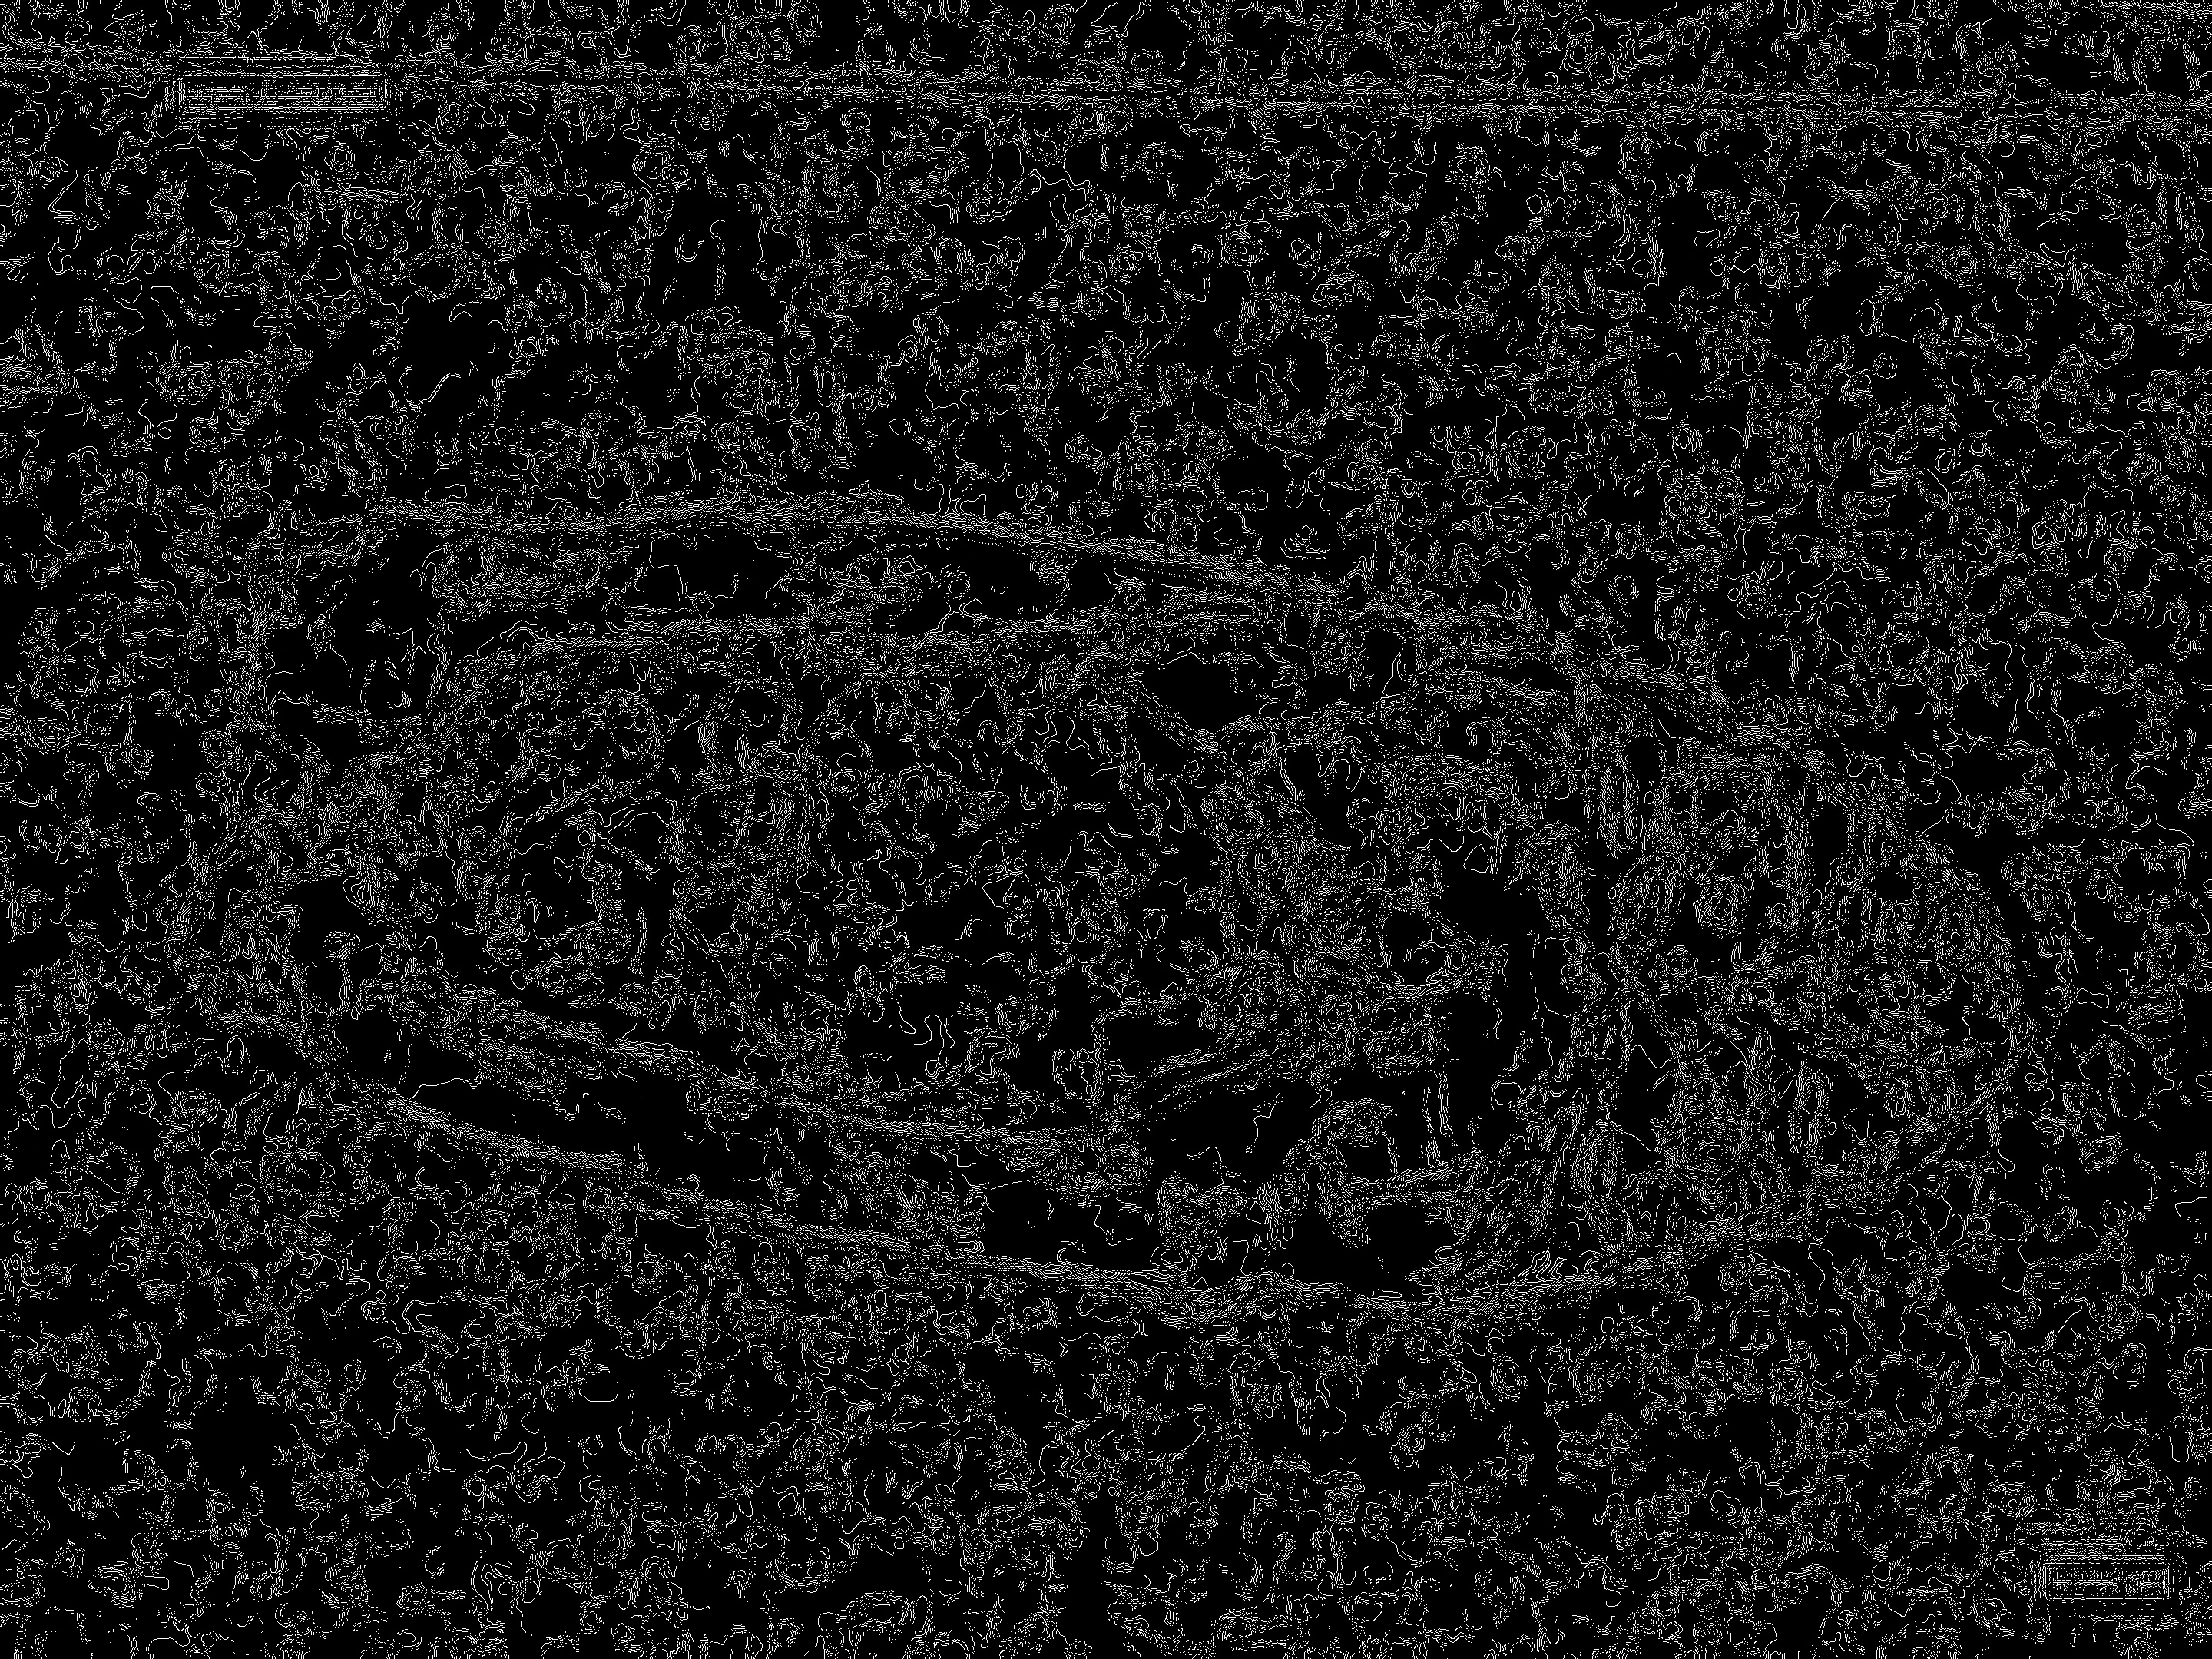
\includegraphics[width=\textwidth]{./fig/gausssian/canny61+2.jpg}
        \caption{canny 2 5}
        \label{fig:canny2_5}
    \end{minipage}
    \begin{minipage}{0.45\textwidth}
        \centering
        \includegraphics[width=\textwidth]{./fig/gausssian/canny61+4.jpg}
        \caption{canny 4 10}
        \label{fig:canny4_10}
    \end{minipage}
\end{figure}

\begin{figure}
    \centering
    \begin{minipage}{0.45\textwidth}
        \centering
        \includegraphics[width=\textwidth]{./fig/gausssian/canny61+6.jpg}
        \caption{canny 6 15}
        \label{fig:canny6_15}
    \end{minipage}
\end{figure}

在三张canny算法的结果中,可见\autoref{fig:canny4_10}的效果最好,其能在保证边缘细节得到大部分保留的情况下,去除了大部分的噪声。因此我们选择canny算法的阈值为4 10。

\textbf{总结}

对比sobel, laplacian和canny算法的结果,sobel算法的效果一般,对于底噪不是能很好的去除,边缘检测效果还算显著。laplacian算法最差,边缘甚至已经不可见,这可能是因为该算法对噪声最敏感。canny算法的效果最好,能够在保证边缘细节的情况下,去除大部分的噪声。因此我们选择canny算法作为图像预处理的方法。

\FloatBarrier


\subsubsection{阈值分割}

考虑到生物组织样本的主体是黄色,石蜡是白色,我们可以通过设置一个阈值,将图像中的白色部分分割出来,那么剩下的就是生物组织部分。在这里使用python的opencv库中进行操作。首先将图像进行对比度增强,增加饱和度,更好的凸显出生物组织的颜色(\autoref{fig:enhanced_image})。之后读取图像的每个像素点,将黄色周围半径15左右的像素点进行保留(约为图像宽的百分之一),其他的色块进行去除。(如\autoref{fig:yellowpic})。

\begin{figure}
    \centering
    \begin{minipage}{0.45\textwidth}
        \centering
        \includegraphics[width=\textwidth]{./fig/threshold/enhanced_image.jpg}
        \caption{enhanced image}
        \label{fig:enhanced_image}
    \end{minipage}
    \begin{minipage}{0.45\textwidth}
        \centering
        \includegraphics[width=\textwidth]{./fig/threshold/yellowpic.jpg}
        \caption{yellow picture}
        \label{fig:yellowpic}
    \end{minipage}
\end{figure}

但是观察发现,这种方法对于生物组织和石蜡的分割效果并不好,因为生物组织在切片过程中会掉落碎片组织,出现在标本各处,进而影响黄色像素点的识别。此时还需要进一步的处理,去除黑色色块。此时只需要将黑色色块进行掩码反转,使其变为白色即可。结果如图\autoref{fig:mask}所示。

\begin{figure}
    \centering
    \begin{minipage}{0.45\textwidth}
        \centering
        \includegraphics[width=\textwidth]{./fig/threshold/final.jpg}
        \caption{final}
        \label{fig:mask}
    \end{minipage}
    \begin{minipage}{0.45\textwidth}
        \centering
        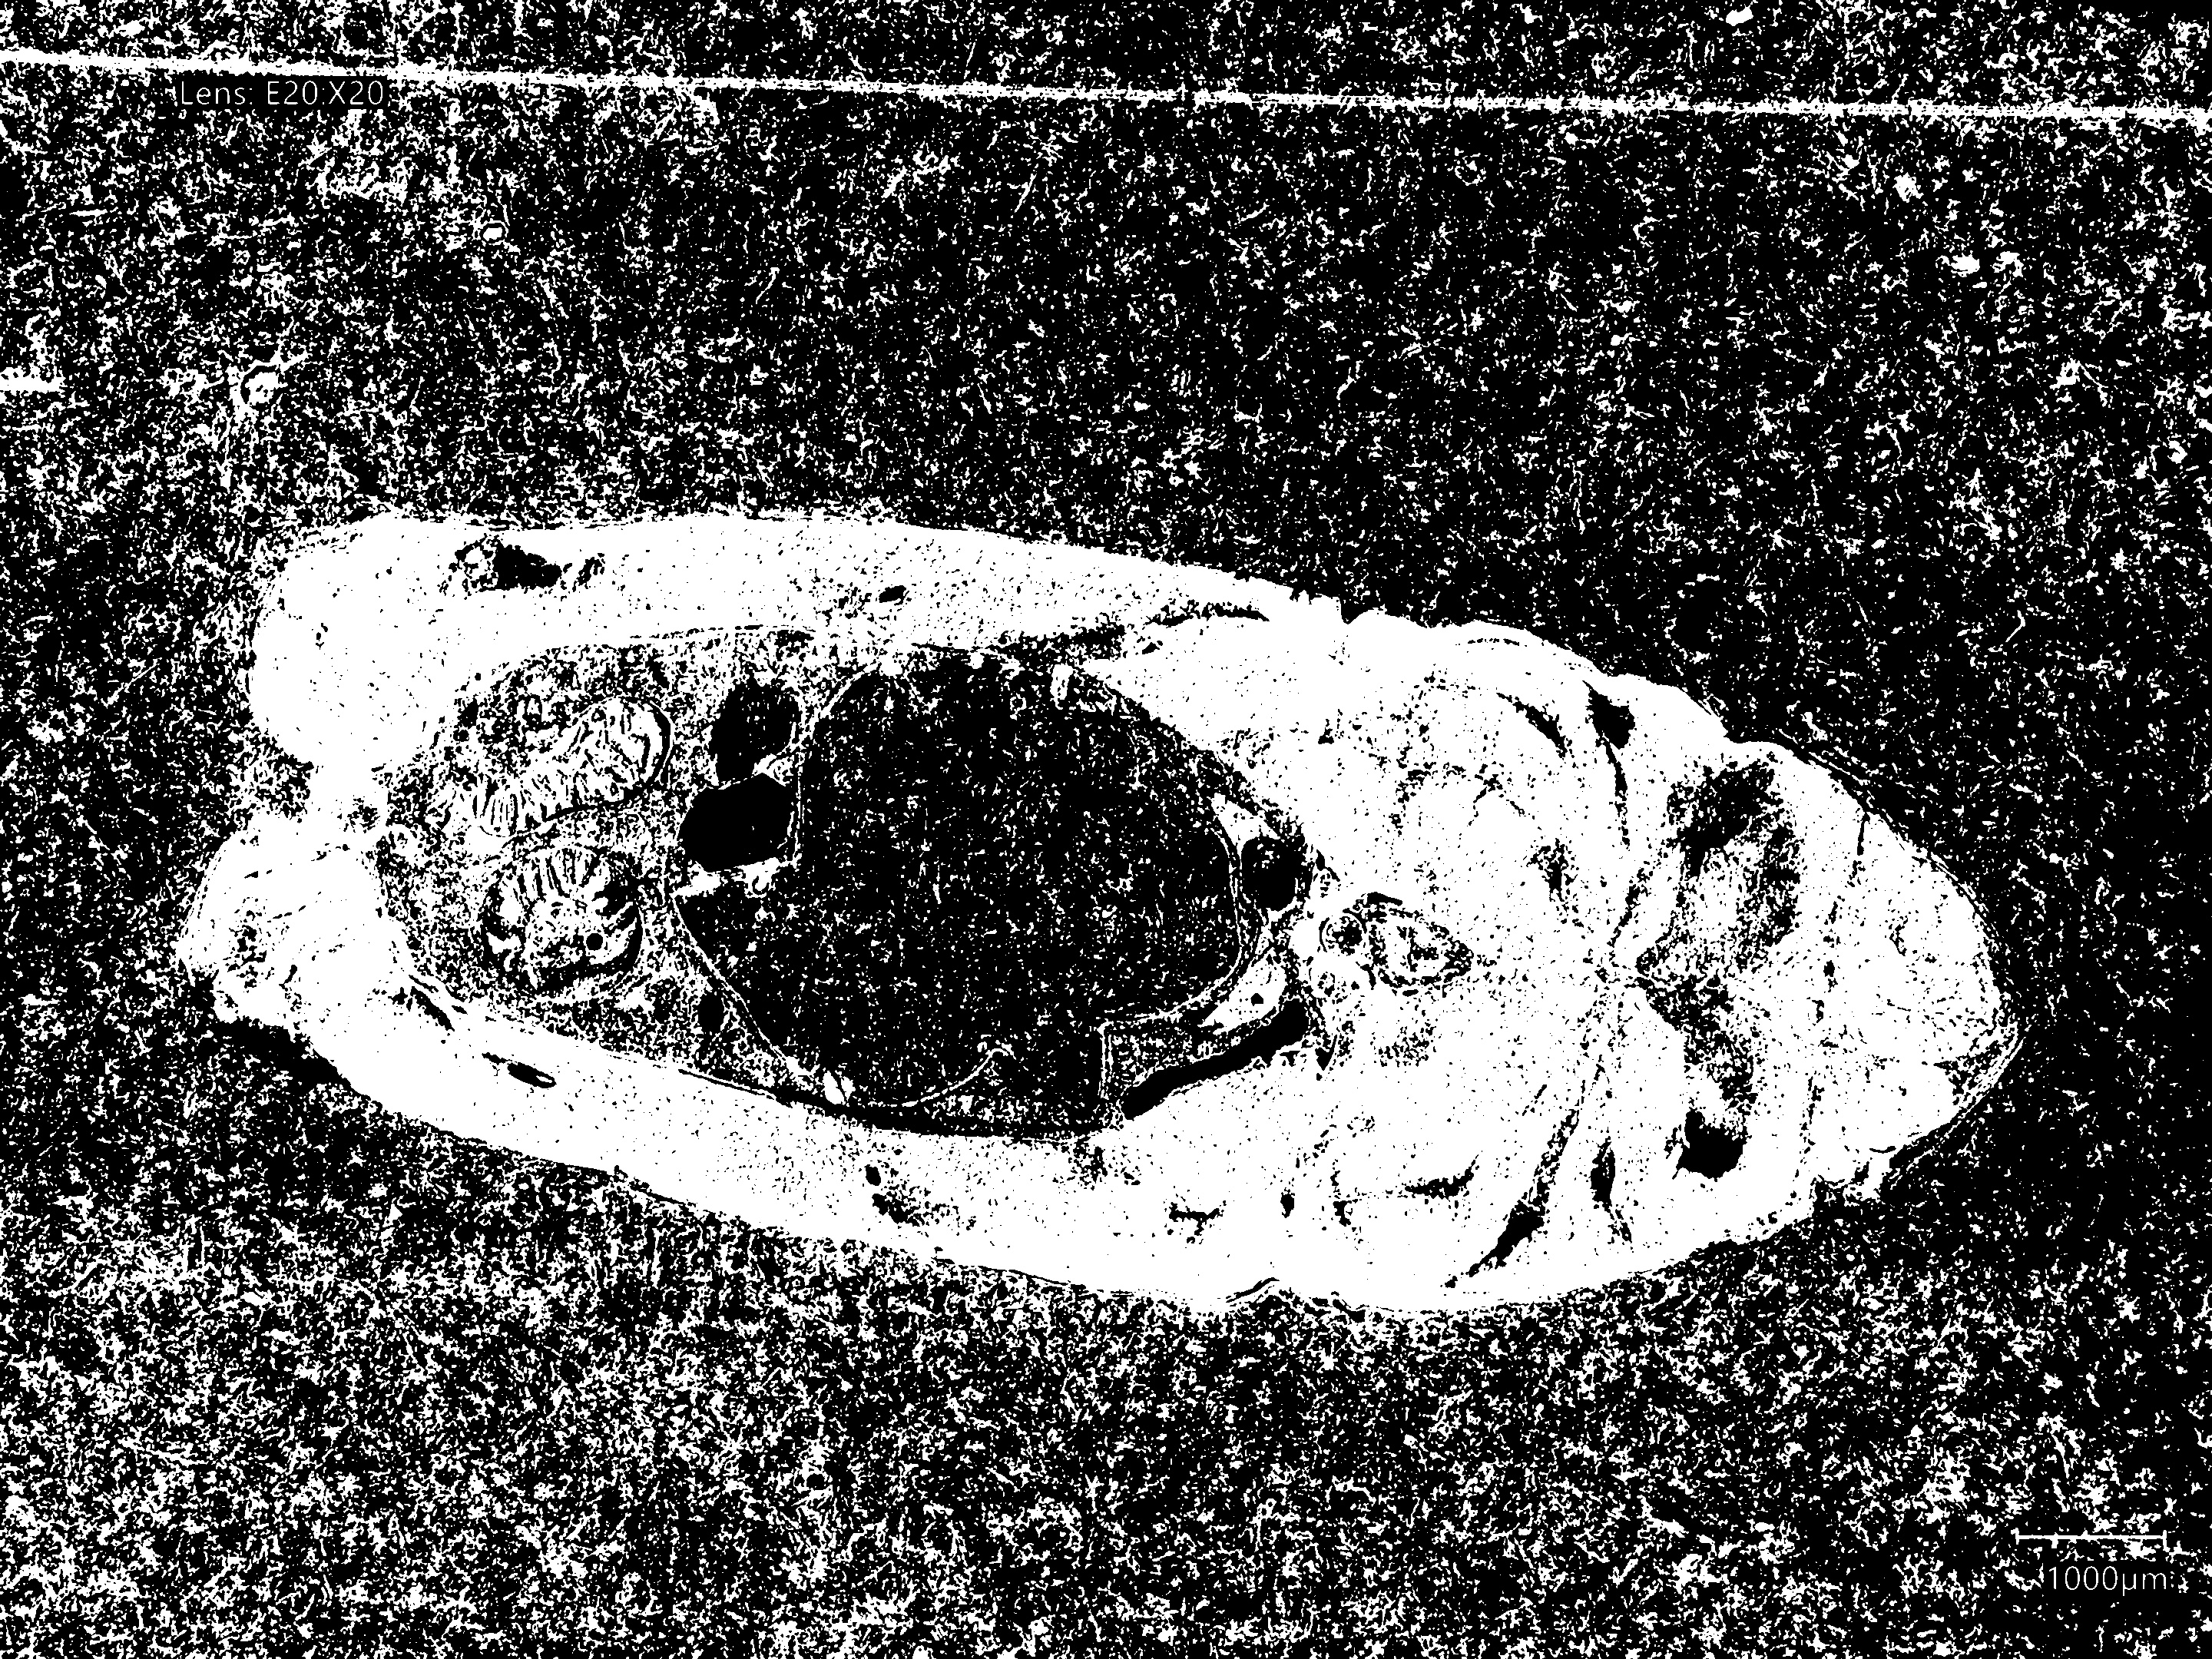
\includegraphics[width=\textwidth]{./fig/threshold/fingerprint.jpg}
        \caption{fingerprint}
        \label{fig:fingerprint}
    \end{minipage}
\end{figure}

\subsubsection{另一种阈值分割方法-指纹算法}
在进行文献综述的时候,发现有一篇论文是基于otsu算法改进的分割方法用于进行指纹分割。考虑到切片样本和指纹都属于生物组织,因此我们尝试使用论文中提到的算法进行分割。结果如图\autoref{fig:fingerprint}所示。

\subsubsection{小结}
根据上文提到的图像预处理方法,我们可以看到,边缘检测和阈值分割的效果都不错,都能够很好的突出生物组织的特征,去除石蜡的干扰。对此我们可以设置三组数据集,分别是经过边缘检测后的图像,经过阈值分割后的图像和经过指纹算法分割后的图像。这三组数据集将作为我们的训练集,用于下一节的模型训练。

\FloatBarrier
\subsection{模型2:预处理图像+简单的cnn网络}

在这里基础模型选用在上一节模型1中表现相对比较好的模型1c。在这里我们将模型1c的输入改为经过预处理后的图像,即边缘检测后的图像,阈值分割后的图像和指纹算法分割后的图像。模型的架构不变,只是输入的数据发生了变化。

\subsubsection{model 2a}

模型2a采用和模型1c同样的架构构成,分别由三个包含32个特征图,卷积核为3*3的卷积层和最大池化层,一个包含256个神经元的全连接层组成。模型的输入为经过\textbf{canny边缘检测}后的图像。

模型训练的准确度和损失如\autoref{fig:model2a_acc}和\autoref{fig:model2a_loss}所示。

\begin{figure}
    \centering
    \begin{minipage}{0.45\textwidth}
        \centering
        \includegraphics[width=\textwidth]{./fig/model2/accuracy2a.eps}
        \caption{Model-2a accuracy}
        \label{fig:model2a_acc}
    \end{minipage}
    \begin{minipage}{0.45\textwidth}
        \centering
        \includegraphics[width=\textwidth]{./fig/model2/loss2a.eps}
        \caption{Model-2a loss}
        \label{fig:model2a_loss}
    \end{minipage}
\end{figure}



\subsubsection{model 2b}

模型2b采用和模型1c同样的架构构成但是模型的输入为经过\textbf{阈值分割}后的图像。

模型训练的准确度和损失如\autoref{fig:model2b_acc}和\autoref{fig:model2b_loss}所示。

\begin{figure}
    \centering
    \begin{minipage}{0.45\textwidth}
        \centering
        \includegraphics[width=\textwidth]{./fig/model2/accuracy2b.eps}
        \caption{Model-2b accuracy}
        \label{fig:model2b_acc}
    \end{minipage}
    \begin{minipage}{0.45\textwidth}
        \centering
        \includegraphics[width=\textwidth]{./fig/model2/loss2b.eps}
        \caption{Model-2b loss}
        \label{fig:model2b_loss}
    \end{minipage}
\end{figure}


\subsubsection{model 2c}

模型2c采用和模型1c同样的架构构成但是模型的输入为经过\textbf{指纹算法分割}后的图像。

模型训练的准确度和损失如\autoref{fig:model2c_acc}和\autoref{fig:model2c_loss}所示。

\begin{figure}
    \centering
    \begin{minipage}{0.45\textwidth}
        \centering
        \includegraphics[width=\textwidth]{./fig/model2/accuracy2c.eps}
        \caption{Model-2c accuracy}
        \label{fig:model2c_acc}
    \end{minipage}
    \begin{minipage}{0.45\textwidth}
        \centering
        \includegraphics[width=\textwidth]{./fig/model2/loss2c.eps}
        \caption{Model-2c loss}
        \label{fig:model2c_loss}
    \end{minipage}
\end{figure}



\subsubsection{小结}
对比模型2a 2b 2c,可以发现模型2a和模型2c在训练步长为5之后就开始收敛,其训练准确度和验证准确度收敛于1和0.8左右。但是损失确仍然较高,这说明模型在训练集上表现良好,但是在验证集上表现欠佳。

模型2b在训练步长为10之后也开始收敛,但是其训练准确度和验证准确度收敛于1和0.8左右,损失收敛于1左右。这说明模型2b表现显著优于模型2a和模型2c。

这可能的原因是模型2a和2c的输入是灰度图,即图像复杂度显著小于彩色图,而模型2b的输入是彩色图,因此在模型提取特征时还能够参考根据色块的rgb值进行提取,故模型2b的表现最好。

但是,在训练过程中,我们发现对于部分图像,经过模型2(特别是2b)的前处理(阈值分割)后,图像的部分重要细节会丢失,进而影响图像标签的准确性。例子如下所示:

\begin{figure}
    \centering
    \begin{minipage}{0.45\textwidth}
        \centering
        \includegraphics[width=\textwidth]{./fig/model2/origin20240205_161427.jpg}
        \caption{origin}
        \label{fig:origin}
    \end{minipage}
    \begin{minipage}{0.45\textwidth}
        \centering
        \includegraphics[width=\textwidth]{./fig/model2/yellow20240205_161427.jpg}
        \caption{yellow}
        \label{fig:yellow}
    \end{minipage}
\end{figure}

\autoref{fig:yellow}是模型2b训练集(经过黄色阈值分割后的图像)中的一张图片,对比原图(\autoref{fig:origin})可以观察发现,原本切片中能够被接受的平行白线被阈值分割算法显著增强了,这有极有可能会影响模型的训练效果,即模型会在一定程度上与horizental line混淆。

此外,经过图像前处理过的图像,还会在一定程度上丢失部分细节,这也会影响模型的训练效果。因此,图像前处理的方法虽然能够在一定程度上提高模型的训练效果,但是也会在一定程度上影响模型的训练效果。因此,我们需要进一步的改进模型,以提高模型的训练效果。

\FloatBarrier
\subsection{模型3:原始图像+迁移学习}

现在我们已经尝试过了简单的cnn网络,以及对图像进行预处理后的cnn网络。既然训练结果不是很理想,那我们为什么不去尝试更大更深的模型? 在这一节,我们尝试使用迁移学习的方法,使用预训练好的大规模深度学习模型,将其迁移到我们的数据集上,以提高模型的训练效果。

正如在第三节methodology里提到的,在这里将使用VGG16,VGG19和InceptionV3三个模型进行迁移学习。这三个模型都是在ImageNet数据集上训练好的模型,具有已经训练好的权重。

在这里为了避免过拟合,不仅使用了原有的早停法,还限制了模型的学习率(1e-5)

model3a是使用VGG16模型进行迁移学习的模型,model3b是使用VGG19模型进行迁移学习的模型,model3c是使用InceptionV3模型进行迁移学习的模型。

\subsubsection{model 3a}
根据VGG16的训练架构,输入层应该为224*224的图像,因此我们需要将图像的分辨率调整为224*224。

模型训练的准确度和损失如\autoref{fig:model3a_acc}和\autoref{fig:model3a_loss}所示

\begin{figure}
    \centering
    \begin{minipage}{0.45\textwidth}
        \centering
        \includegraphics[width=\textwidth]{./fig/model3/accuracy3a.eps}
        \caption{Model-3a accuracy}
        \label{fig:model3a_acc}
    \end{minipage}
    \begin{minipage}{0.45\textwidth}
        \centering
        \includegraphics[width=\textwidth]{./fig/model3/loss3a.eps}
        \caption{Model-3a loss}
        \label{fig:model3a_loss}
    \end{minipage}
\end{figure}

\subsubsection{model 3b}
VGG19和VGG16相比只是在中间增加了3个额外的卷积层,其他与VGG16相同。模型训练的准确度和损失如\autoref{fig:model3b_acc}和\autoref{fig:model3b_loss}所示

\begin{figure}
    \centering
    \begin{minipage}{0.45\textwidth}
        \centering
        \includegraphics[width=\textwidth]{./fig/model3/accuracy3b.eps}
        \caption{Model-3b accuracy}
        \label{fig:model3b_acc}
    \end{minipage}
    \begin{minipage}{0.45\textwidth}
        \centering
        \includegraphics[width=\textwidth]{./fig/model3/loss3b.eps}
        \caption{Model-3b loss}
        \label{fig:model3b_loss}
    \end{minipage}
\end{figure}

\subsubsection{model 3c}
InceptionV3是一个相对于VGG16和VGG19更加复杂的模型,其在训练过程中引入了Inception模块,能够更好的提取图像的特征。其顶层的输入面积为299*299.
模型训练的准确度和损失如下\autoref{fig:model3c_acc}和\autoref{fig:model3c_loss}所示

\begin{figure}
    \centering
    \begin{minipage}{0.45\textwidth}
        \centering
        \includegraphics[width=\textwidth]{./fig/model3/accuracy3c.eps}
        \caption{Model-3c accuracy}
        \label{fig:model3c_acc}
    \end{minipage}
    \begin{minipage}{0.45\textwidth}
        \centering
        \includegraphics[width=\textwidth]{./fig/model3/loss3c.eps}
        \caption{Model-3c loss}
        \label{fig:model3c_loss}
    \end{minipage}
\end{figure}

注意到模型3c的验证准确度上依旧保持上升趋势,验证损失也在不断下降,这说明模型3c的训练可能还没到达最佳状态,模型欠拟合,需要进一步增加步长。

模型3d是对模型3c的改进,增加步长为1000(原来为100),模型训练的准确度和损失如\autoref{fig:model3d_acc}和\autoref{fig:model3d_loss}所示

\begin{figure}
        \centering
        \begin{minipage}{0.45\textwidth}
            \centering
            \includegraphics[width=\textwidth]{./fig/model3/accuracy3d.eps}
            \caption{Model-3d accuracy}
            \label{fig:model3d_acc}
        \end{minipage}
        \begin{minipage}{0.45\textwidth}
            \centering
            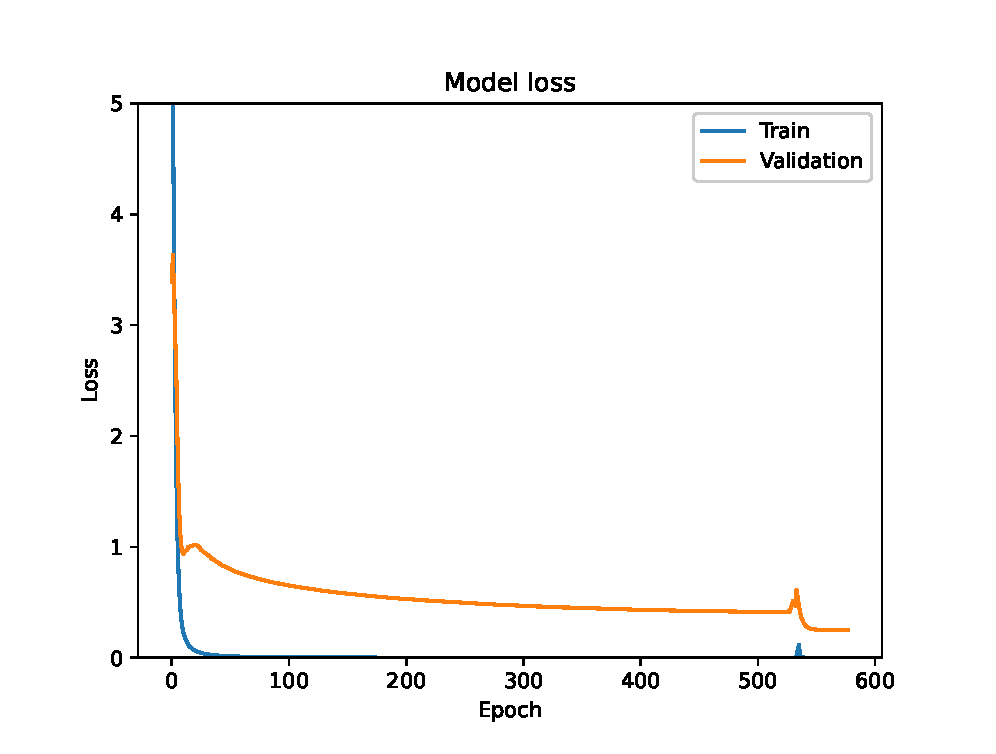
\includegraphics[width=\textwidth]{./fig/model3/loss3d.eps}
            \caption{Model-3d loss}
            \label{fig:model3d_loss}
        \end{minipage}
\end{figure}

\subsubsection{小结}

对比VGG16,VGG19和InceptionV3三个模型,可以发现InceptionV3的训练效果最好,其训练准确度和验证准确度收敛于1和0.9左右,损失收敛于0.5左右。这说明InceptionV3模型的训练效果最好,其泛化能力最强。

\subsection{模型选择总结}
横向对比模型1,模型2和模型3,可以发现模型3的训练效果最好。特别是模型3d。究其原因,可能是因为模型3是基于大规模图像识别的超深卷积网络,其在训练过程中能够更好的提取图像的特征,构建自己的特征空间。值得注意的是,模型3d,属于InceptionV3,在架构上具有模块化的设计,包括了多个“inception模块”。其包含了多尺度的卷积层,同时在同一层内并行运行。
在特征提取上,Inception模块可以在同一层内捕捉不同尺度的特征,使得网络能够自适应地选择更合适的特征表示。在处理深度上,InceptionV3利用批量标准化和残差连接来帮助训练深层网络,可以显著解决梯度消失的问题。

因此,我们选择模型3d作为我们的最终模型,用于后续的进一步应用和测试。

